\documentclass[a4paper]{article}

\usepackage[polish]{babel}
\usepackage[utf8]{inputenc}
\usepackage[T1]{fontenc}
\usepackage{graphicx}
\graphicspath{ {./aem/} }
\usepackage[colorinlistoftodos]{todonotes}
\usepackage[procnames]{listings}
\usepackage{ucs}
\usepackage{float}
\usepackage{hyperref}
\usepackage{makecell}


\lstset{
    basicstyle=\ttfamily\small,
    numberstyle=\footnotesize,
    numbers=left,
	frame=single,
    tabsize=2,
    rulecolor=\color{black!30},
    breaklines=true,
    breakatwhitespace=true,
    inputencoding=utf8x,
    extendedchars=\true,
    literate={ą}{{\k{a}}}1
             {Ą}{{\k{A}}}1
             {ę}{{\k{e}}}1
             {Ę}{{\k{E}}}1
             {ó}{{\'o}}1
             {Ó}{{\'O}}1
             {ś}{{\'s}}1
             {Ś}{{\'S}}1
             {ł}{{\l{}}}1
             {Ł}{{\L{}}}1
             {ż}{{\.z}}1
             {Ż}{{\.Z}}1
             {ź}{{\'z}}1
             {Ź}{{\'Z}}1
             {ć}{{\'c}}1
             {Ć}{{\'C}}1
             {ń}{{\'n}}1
             {Ń}{{\'N}}1
}

\title{Problem komiwojażera}

\author{Adrian Stępień i Wojciech Młyńczak}

\begin{document}

\maketitle

\section{Zadanie 2}

\subsection{Opis zadania}

Zadanie polega na implementacji lokalnego przeszukiwania dla zmodyfikowane problemu komiwojażera. Lokalne przeszukiwanie my być zaimplementowane w wersjach stromej i zachłannej z dwoma różnym rodzajami sąsiedztwa.

\subsection{Opis zaimplementowanych algorytmów}

\subsubsection{Algorytm lokalnego przeszukiwania w wersji zachłannej dla zamiany wierzchołków}

\begin{lstlisting}
Wygeneruj losowe rozwiązanie.
Dopóki nowe rozwiązanie jest lepsze:
    Oznacz, że nowe rozwiązanie jest gorsze.
    Wygeneruj losową serię.
    Dla każdego punktu w serii:
        Wygeneruj drugą losową serię.
        Dla każdego punktu w drugiej losowej serii:
            Jeżeli wybrany punkt jest taki sam jak punkt z pierwszej serii, to przejdź do następnego punktu z drugiej serii.
            Oblicz deltę.
            Jeżeli delta jest mniejsza od 0:
                Zamień punkt z rozwiązania wskazany, przez pierwszą losową serię, na punkt z drugiej serii.
                Oznacz, że nowe rozwiązanie jest lepsze i przejdź do pętli zewnętrznej.
\end{lstlisting}

\subsubsection{Algorytm lokalnego przeszukiwania w wersji stromej dla zamiany wierzchołków}

\begin{lstlisting}
Wygeneruj losowe rozwiązanie.
Dopóki nowe rozwiązanie jest lepsze:
    Oznacz, że nowe rozwiązanie jest gorsze.
    Wyzeruj najlepszą deltę i najlepsze punkty do zamiany.
    Wygeneruj losową serię.
    Dla każdego punktu w serii:
        Wygeneruj drugą losową serię.
        Dla każdego punktu w drugiej losowej serii:
            Jeżeli wybrany punkt jest taki sam jak punkt z pierwszej serii, to przejdź do następnego punktu z drugiej serii.
            Oblicz deltę.
            Jeżeli delta jest lepsza od najlepszej delty:
                Zamień najlepszą deltę na obliczoną deltę.
                Zamień znalezione punkty z obecnymi punktami do zamiany.
                Oznacz, że nowe rozwiązanie jest lepsze.
    Jeżeli najlepsza delta jest mniejsza od 0, to zamień znalezione dwa punkty ze sobą.
\end{lstlisting}

\subsubsection{Algorytm lokalnego przeszukiwania w wersji zachłannej dla zamiany krawędzi}

\begin{lstlisting}
Wygeneruj losowe rozwiązanie.
Dopóki nowe rozwiązanie jest lepsze:
    Oznacz, że nowe rozwiązanie jest gorsze.
    Wyzeruj najlepszą deltę i najlepsze punkty do zamiany.
    Wylosuj czy następuje wymiana wierzchołków pozatrasowych czy krawędzi wewnątrz trasowych
    Jeżeli wylosowano wymianę wierzchołków pozatrasowych
    	Wygeneruj losową serię.
    	Dla każdego punktu w serii:
        	Oblicz dystans aktualnego rozwiązania.
        	Wygeneruj drugą losową serię bez punktów z aktualnego rozwiązania.
        	Dla każdego punktu w drugiej losowej serii:
            	Jeżeli wybrany punkt jest taki sam jak punkt z pierwszej serii, to przejdź do następnego punktu z drugiej serii.
            	Oblicz deltę.
            	Jeżeli delta jest mniejsza od zera
                	Zamień znalezione dwa punkty ze sobą.
                	Oznacz, że nowe rozwiązanie jest lepsze i przejdź do pętli zewnętrznej.
	Jeżeli wylosowano wymianę krawędzi
    	Wygeneruj losową serię.
    	Dla każdej krawędzi w serii:
        	Wygeneruj drugą losową serię.
        	Dla każdej krawędzi w drugiej losowej serii:
            	Jeżeli wybrana krawędź jest taka sama jak krawędź z pierwszej serii lub sąsiadują za sobą, to przejdź do następnej krawędzi z drugiej serii.
            	Oblicz deltę.
            	Jeżeli delta jest mniejsza od zera
                	Zamień znalezione dwie krawędzie.
                	Oznacz, że nowe rozwiązanie jest lepsze i przejdź do pętli zewnętrznej.
\end{lstlisting}

\subsubsection{Algorytm lokalnego przeszukiwania w wersji stromej dla zamiany krawędzi}

\begin{lstlisting}
Wygeneruj losowe rozwiązanie.
Dopóki nowe rozwiązanie jest lepsze:
    Oznacz, że nowe rozwiązanie jest gorsze.
    Wyzeruj najlepszą deltę i najlepsze punkty do zamiany.
    Wygeneruj losową serię.
    Dla każdego punktu w serii:
        Oblicz dystans aktualnego rozwiązania.
        Wygeneruj drugą losową serię bez punktów z aktualnego rozwiązania.
        Dla każdego punktu w drugiej losowej serii:
            Jeżeli wybrany punkt jest taki sam jak punkt z pierwszej serii, to przejdź do następnego punktu z drugiej serii.
            Oblicz deltę.
            Jeżeli delta jest lepsza od najlepszej delty:
                Zamień najlepszą deltę na obliczoną deltę.
                Zamień znalezione punkty z obecnymi punktami do zamiany.
                Oznacz, że nowe rozwiązanie jest lepsze.
    Wygeneruj losową serię.
    Dla każdego punktu w serii:
        Wygeneruj drugą losową serię.
        Dla każdej krawędzi w drugiej losowej serii:
            Jeżeli wybrana krawędź jest taka sama jak krawędź z pierwszej serii lub sąsiadują za sobą, to przejdź do następnej krawędzi z drugiej serii.
            Oblicz deltę.
            Jeżeli delta jest lepsza od najlepszej delty:
                Zamień najlepszą deltę na obliczoną deltę.
                Zamień znalezione punkty z obecnymi punktami do zamiany.
                Oznacz, że nowe rozwiązanie jest lepsze.
    Jeżeli najlepsza delta jest mniejsza od 0, to zamień znalezione dwa punkty ze sobą.
\end{lstlisting}

\subsubsection{Sposób randomizacji kolejności przeglądania}

W algorytmie wykorzystano randomizację kolejności przeszukiwania. Są to wszystkie operacje opisane jako generowanie serii. Polegają one na wygenerowaniu indeksów krawędzi lub punktów (w zależności od tego co będzie wymieniane) w losowej kolejności. Następnie, gdy przeglądane są kolejne punkty lub krawędzie są one pobierane z wygenerowanej serii, dzięki czemu kolejność przeglądania za każdą iteracją pętli głównej jest inna. 

\subsection{Wyniki pomiarów}

\begin{center}
	\hspace*{-2.75cm}
	\begin{tabular}{ l | l | l | l | l | l | l }
		\textbf{Pomiar} & \textbf{\makecell{Wartość \\ średnia}} & \textbf{\makecell{Wartość \\ minimalna}} & \textbf{\makecell{Wartość \\ maksymalna}} & \textbf{\makecell{Średni \\ czas [ms]}} & \textbf{\makecell{Minimalny \\ czas [ms]}} & \textbf{\makecell{Maksymalny \\ czas [ms]}} \\
		\hline
		\makecell{Zamiana wierzchołków \\ w wersji stromej \\ dla kroA100}    & 18116.54 & 14316.00 & 16646.00 & 701 & 436 &  925 \\
		\makecell{Zamiana wierzchołków \\ w wersji zachłannej \\ dla kroA100} & 16747.61 & 13694.00 & 16207.00 & 116 &  71 &  224 \\
		\makecell{Zamiana krawędzi \\ w wersji stromej \\ dla kroA100}        & 12545.69 & 10769.00 & 11889.00 & 685 & 517 &  858 \\
		\makecell{Zamiana krawędzi \\ w wersji zachłannej \\ dla kroA100}     & 13469.44 & 11091.00 & 14262.00 &  56 &  26 &   92 \\
		\makecell{Zamiana wierzchołków \\ w wersji stromej \\ dla kroB100}    & 17721.50 & 14033.00 & 15635.00 & 717 & 504 & 1108 \\
		\makecell{Zamiana wierzchołków \\ w wersji zachłannej \\ dla kroB100} & 16873.84 & 12300.00 & 15330.00 & 106 &  72 &  158 \\
		\makecell{Zamiana krawędzi \\ w wersji stromej \\ dla kroB100}        & 12541.73 & 11199.00 & 13471.00 & 665 & 502 &  835 \\
		\makecell{Zamiana krawędzi \\ w wersji zachłannej \\ dla kroB100}     & 13261.47 & 11477.00 & 13227.00 &  60 &  25 &  115 \\
	\end{tabular}
	\hspace*{-2.75cm}
\end{center}

\subsection{Wizualizacje najlepszych rozwiązań}

\subsubsection{Zamiana wierzchołków w wersji stromej dla kroA100}

\begin{figure}[H]
\centering
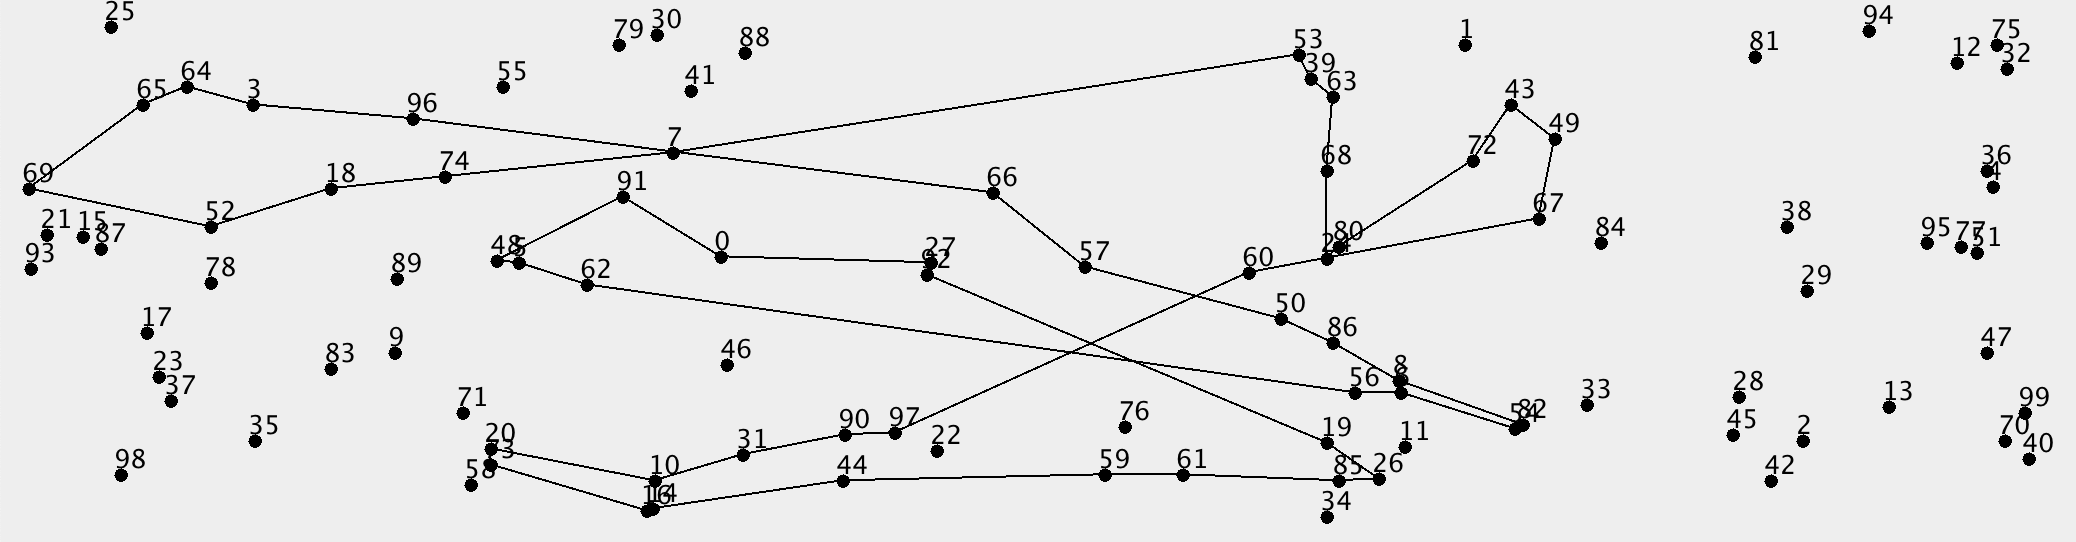
\includegraphics[width=\textwidth]{lab2/kroA_steepest_points}
\caption{Zamiana wierzchołków w wersji stromej dla kroA100}
\end{figure}

\subsubsection{Zamiana wierzchołków w wersji zachłannej dla kroA100}

\begin{figure}[H]
\centering
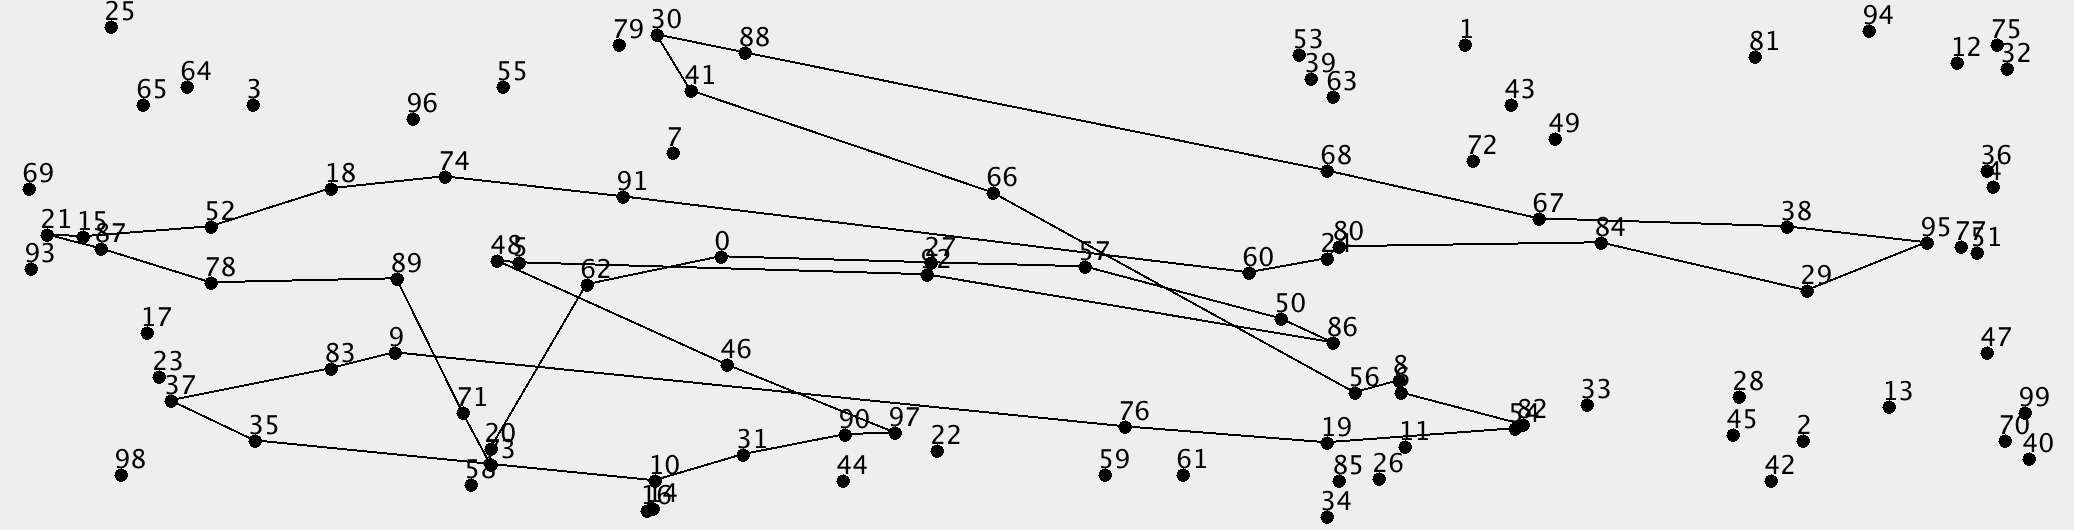
\includegraphics[width=\textwidth]{lab2/kroA_greedy_points}
\caption{Zamiana wierzchołków w wersji zachłannej dla kroA100}
\end{figure}

\subsubsection{Zamiana krawędzi w wersji stromej dla kroA100}

\begin{figure}[H]
\centering
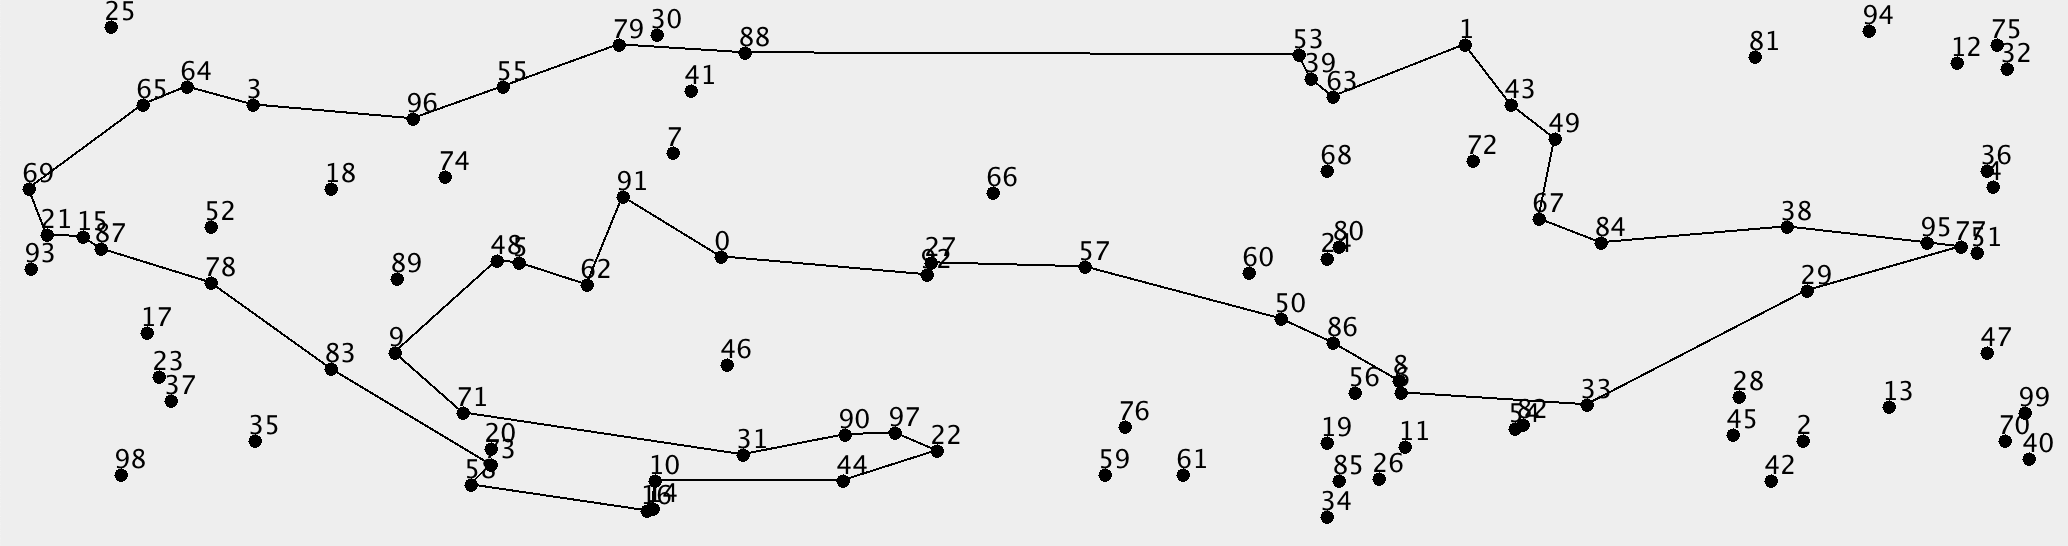
\includegraphics[width=\textwidth]{lab2/kroA_steepest_corners}
\caption{Zamiana krawędzi w wersji stromej dla kroA100}
\end{figure}

\subsubsection{Zamiana krawędzi w wersji zachłannej dla kroA100}

\begin{figure}[H]
\centering
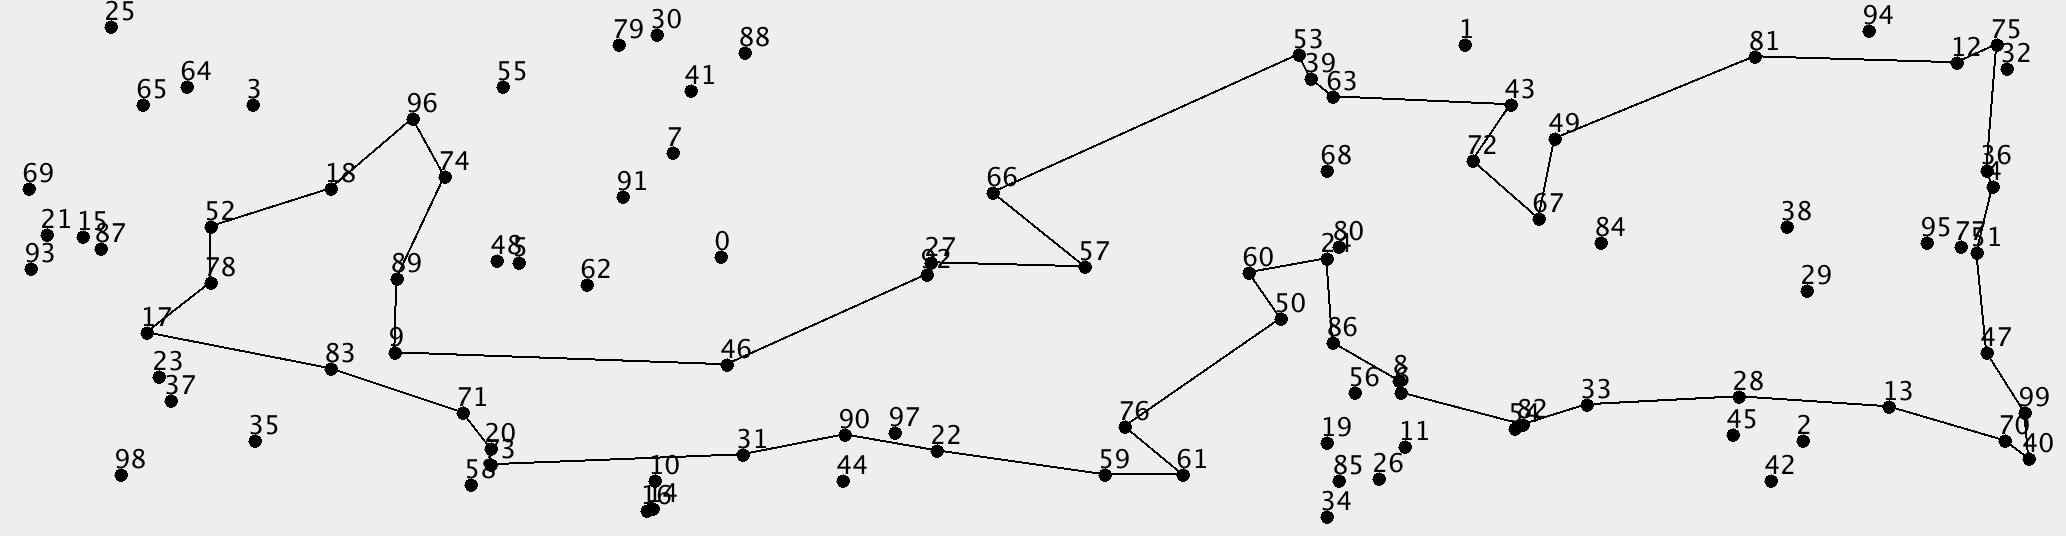
\includegraphics[width=\textwidth]{lab2/kroA_greedy_corners}
\caption{Zamiana krawędzi w wersji zachłannej dla kroA100}
\end{figure}

\subsubsection{Zamiana wierzchołków w wersji stromej dla kroB100}

\begin{figure}[H]
\centering
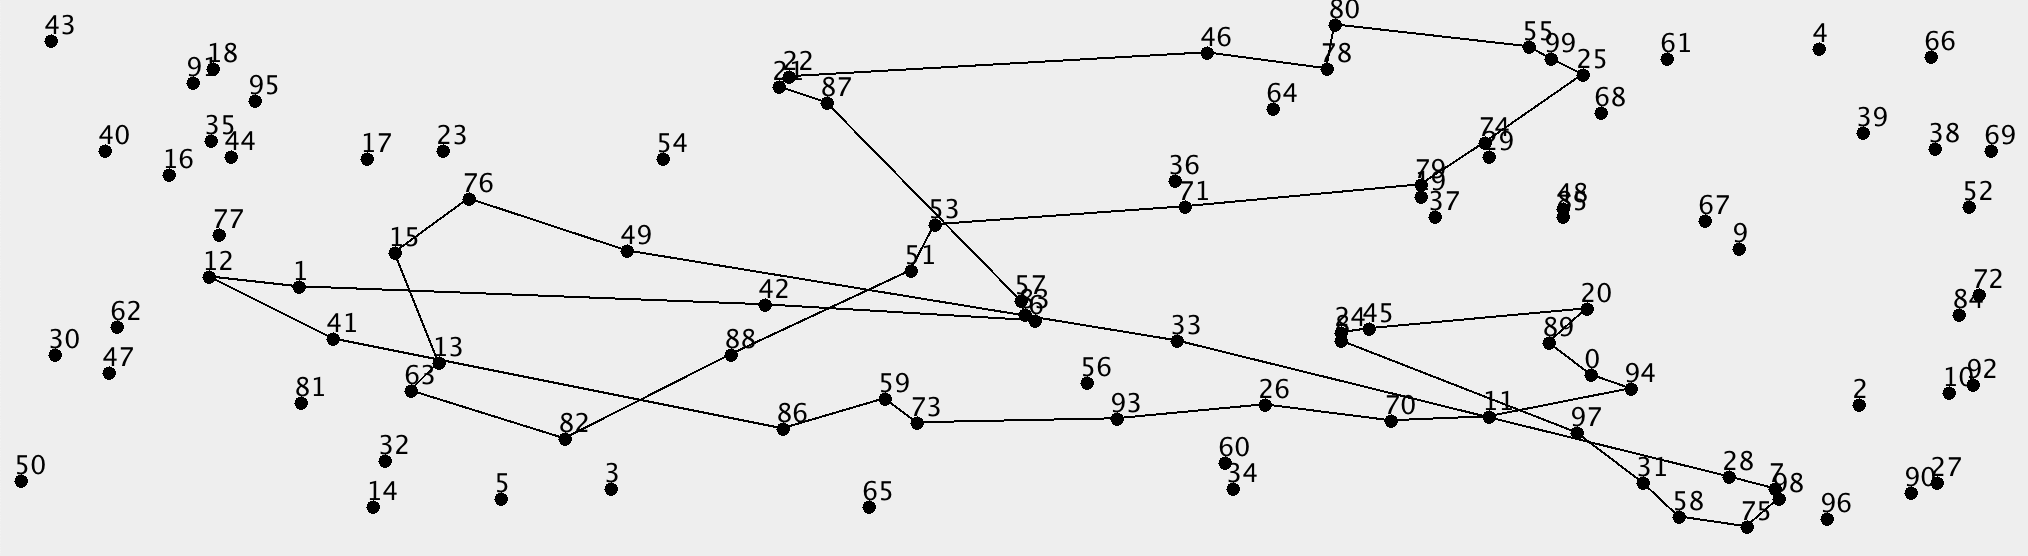
\includegraphics[width=\textwidth]{lab2/kroB_steepest_points}
\caption{Zamiana wierzchołków w wersji stromej dla kroB100}
\end{figure}

\subsubsection{Zamiana wierzchołków w wersji zachłannej dla kroB100}

\begin{figure}[H]
\centering
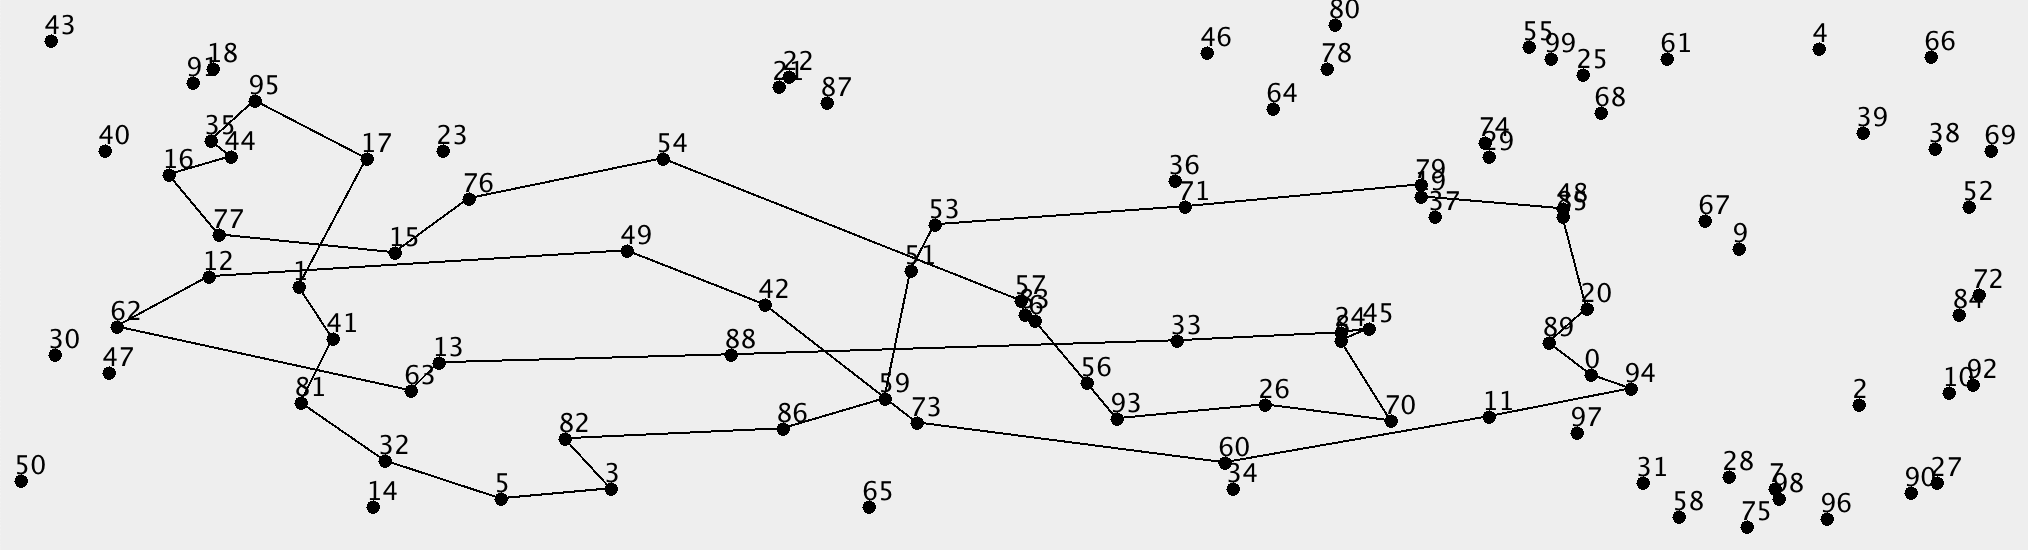
\includegraphics[width=\textwidth]{lab2/kroB_greedy_points}
\caption{Zamiana wierzchołków w wersji zachłannej dla kroB100}
\end{figure}

\subsubsection{Zamiana krawędzi w wersji stromej dla kroB100}

\begin{figure}[H]
\centering
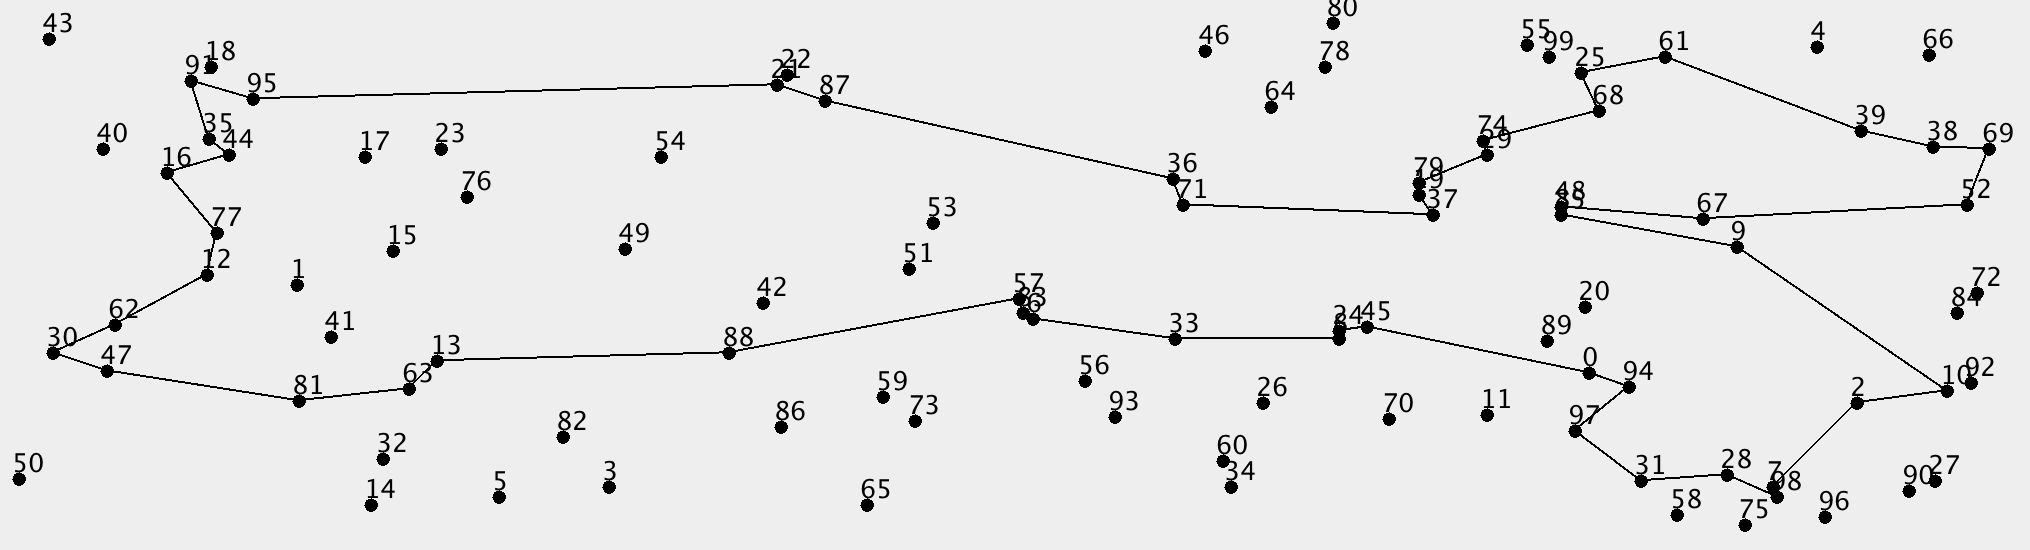
\includegraphics[width=\textwidth]{lab2/kroB_steepest_corners}
\caption{Zamiana krawędzi w wersji stromej dla kroB100}
\end{figure}

\subsubsection{Zamiana krawędzi w wersji zachłannej dla kroB100}

\begin{figure}[H]
\centering
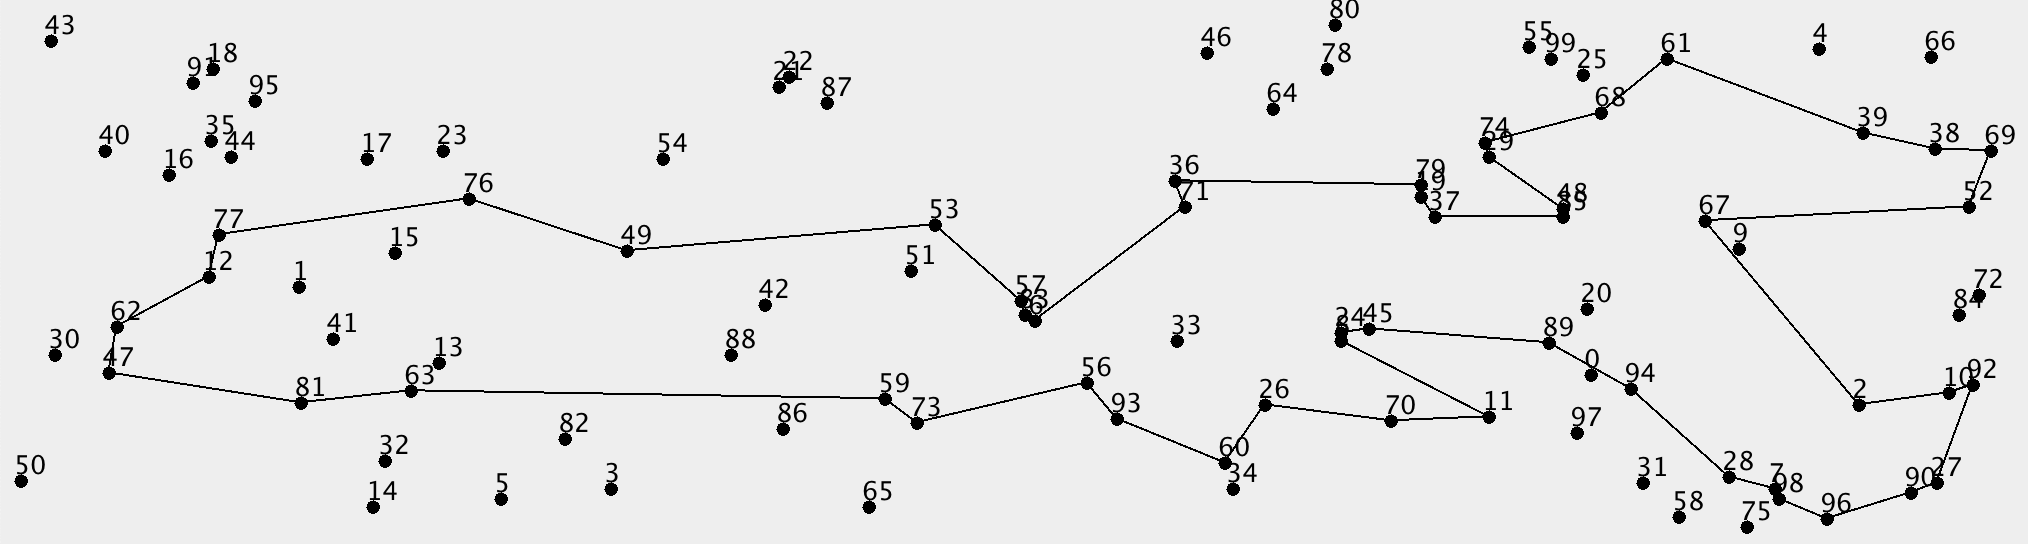
\includegraphics[width=\textwidth]{lab2/kroB_greedy_corners}
\caption{Zamiana krawędzi w wersji zachłannej dla kroB100}
\end{figure}

\subsection{Wnioski}

Z wymienionych wyżej pomiarów można wywnioskować, że dla podanych warunków problemu zamiana kolejności krawędzi dla obu typów algorytmu daje dużo lepsze wyniki niż wymiana wierzchołków. Moża również zaobserwować, że wersja zachłanna dla zamiany wierzchołków daje średnio lepsze wyniki od wersji stromej. Dla zamiany kolejności krawędzi rozwiązania wyniki są odwrotne - wersja stroma daje średnio lepsze rezultaty od wersji zachłannej. Wersja stroma ma o wiele większe czasy wykonywania z powodu, że musi zawsze przeszukiwać całe rozwiązanie w poszukiwaniu najlepszego ruchu, a wersja zachłanna wybiera pierwszy poprawiający rozwiązanie ruch. 

\section{Zadanie 1}

\subsection{Opis zadania}

\paragraph{}
Rozważany problem to zmodyfikowany problem komiwojażera. Dany jest zbiór wierzchołków i macierz odległości pomiędzy każdą parą wierzchołków. Celem zadania jest znalezienie najkrótszej ścieżki zamkniętej przechodzącą przez 50\% wszystkich wierzchołków (w przypadku nieparzystej liczby wierzchołków liczba jest zaokrąglana w górę).

\subsection{Opis zaimplementowanych algorytmów}

\subsubsection{Algorytm zachłanny greedy cycle}

\begin{lstlisting}
Wybierz pierwszy punkt.
Wybierz drugi punkt leżący najbliżej pierwszego.
Jeżeli nie dodałeś wszystkich punktów:
	Dla pozostałych wolnych punktów:
		Dla każdej krawędzi w aktualnym rozwiązaniu:
			Oblicz koszt dodania punktu do rozwiązania w danej krawędzi.
			Sprawdź czy to jest najlepsze rozwiązanie w danym momencie.
	Dodaj znaleziony najlepszy punkt w wybranej krawędzi do cyklu.
\end{lstlisting}

\subsubsection{Algorytm z żalem oparty o 1-żal}

\begin{lstlisting}
Wybierz pierwszy punkt.
Wybierz drugi punkt leżący najbliżej pierwszego.
Jeżeli nie dodałeś wszystkich punktów:
	Dla pozostałych wolnych punktów:
		Dla każdej krawędzi w aktualnym rozwiązaniu:
			Oblicz koszt dodania punktu do rozwiązania w danej krawędzi.
			Dodaj punkt do listy potencjalnych rozwiązań wraz z kosztem dodania.
		Oblicz żal dla danego punktu
	W liście potencjalnych rozwiązań znajdź rozwiązanie z największym żalem.
	Dodaj znalezione rozwiązanie z największym żalem do cyklu.
\end{lstlisting}

\subsection{Wyniki pomiarów}

\subsubsection{Algorytm zachłanny dla problemu kroA100}

\begin{center}
	\begin{tabular}{ l | l }
		\textbf{Pomiar} & \textbf{Wynik} \\
		\hline
		Wartość średnia    & 12898.45 \\
		Wartość minimalna  & 11325.00 \\
		Wartość maksymalna & 14067.00 \\
	\end{tabular}
\end{center}

\subsubsection{Algorytm oparty o żal dla problemu kroA100}

\begin{center}
	\begin{tabular}{ l | l }
		\textbf{Pomiar} & \textbf{Wynik} \\
		\hline
		Wartość średnia    & 16879.11 \\
		Wartość minimalna  & 14456.00 \\
		Wartość maksymalna & 17899.00 \\
	\end{tabular}
\end{center}

\subsubsection{Algorytm zachłanny dla problemu kroB100}

\begin{center}
	\begin{tabular}{ l | l }
		\textbf{Pomiar} & \textbf{Wynik} \\
		\hline
		Wartość średnia    & 12710.59 \\
		Wartość minimalna  & 10240.00 \\
		Wartość maksymalna & 11320.00 \\
	\end{tabular}
\end{center}

\subsubsection{Algorytm oparty o żal dla problemu kroB100}

\begin{center}
	\begin{tabular}{ l | l }
		\textbf{Pomiar} & \textbf{Wynik} \\
		\hline
		Wartość średnia    & 17245.51 \\
		Wartość minimalna  & 15547.00 \\
		Wartość maksymalna & 16965.00 \\
	\end{tabular}
\end{center}

\subsection{Wizualizacje najlepszych rozwiązań}

\subsubsection{Algorytm zachłanny dla problemu kroA100}

\begin{figure}[H]
\centering
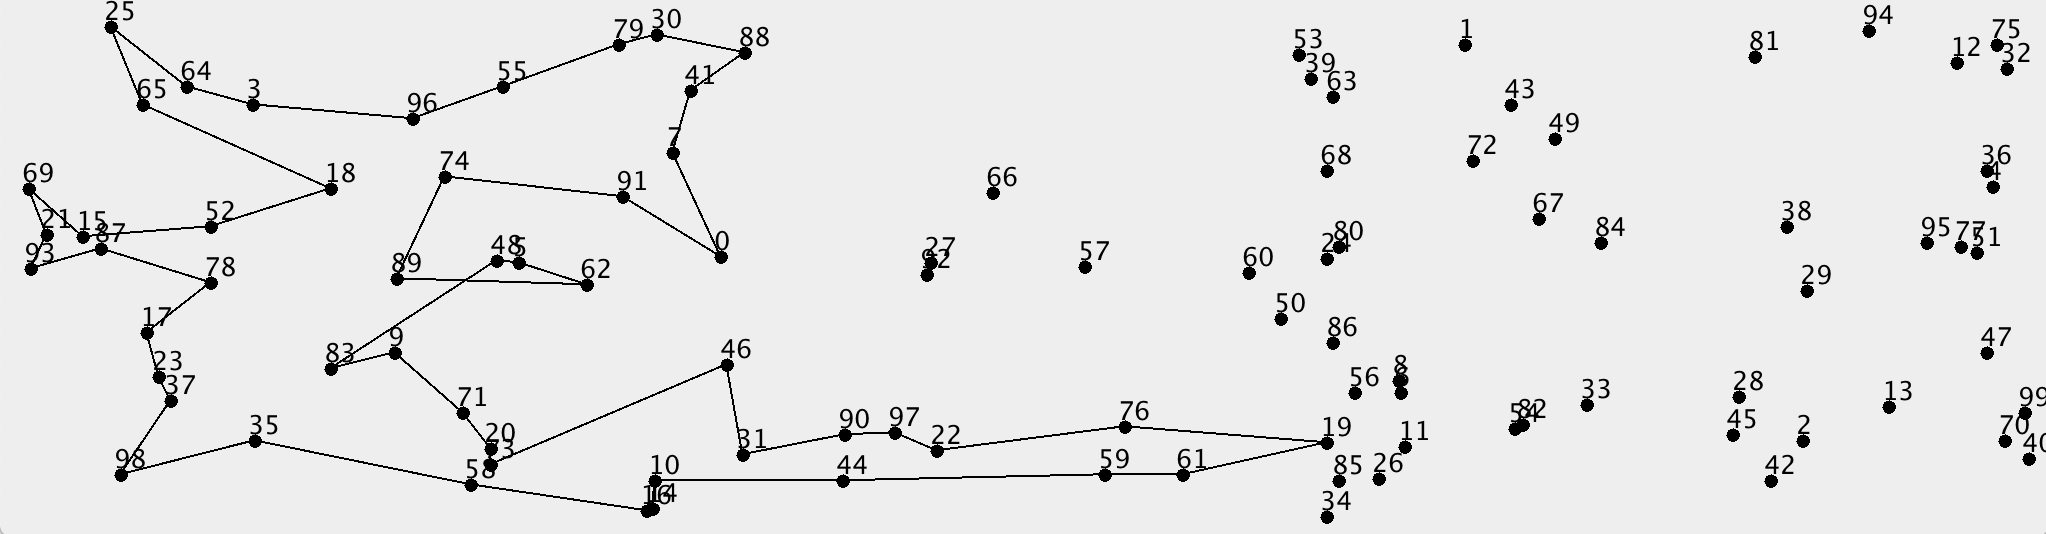
\includegraphics[width=\textwidth]{lab1/kroA_greedy}
\caption{Algorytm zachłanny dla problemu kroA100}
\end{figure}

\subsubsection{Algorytm oparty o żal dla problemu kroA100}

\begin{figure}[H]
\centering
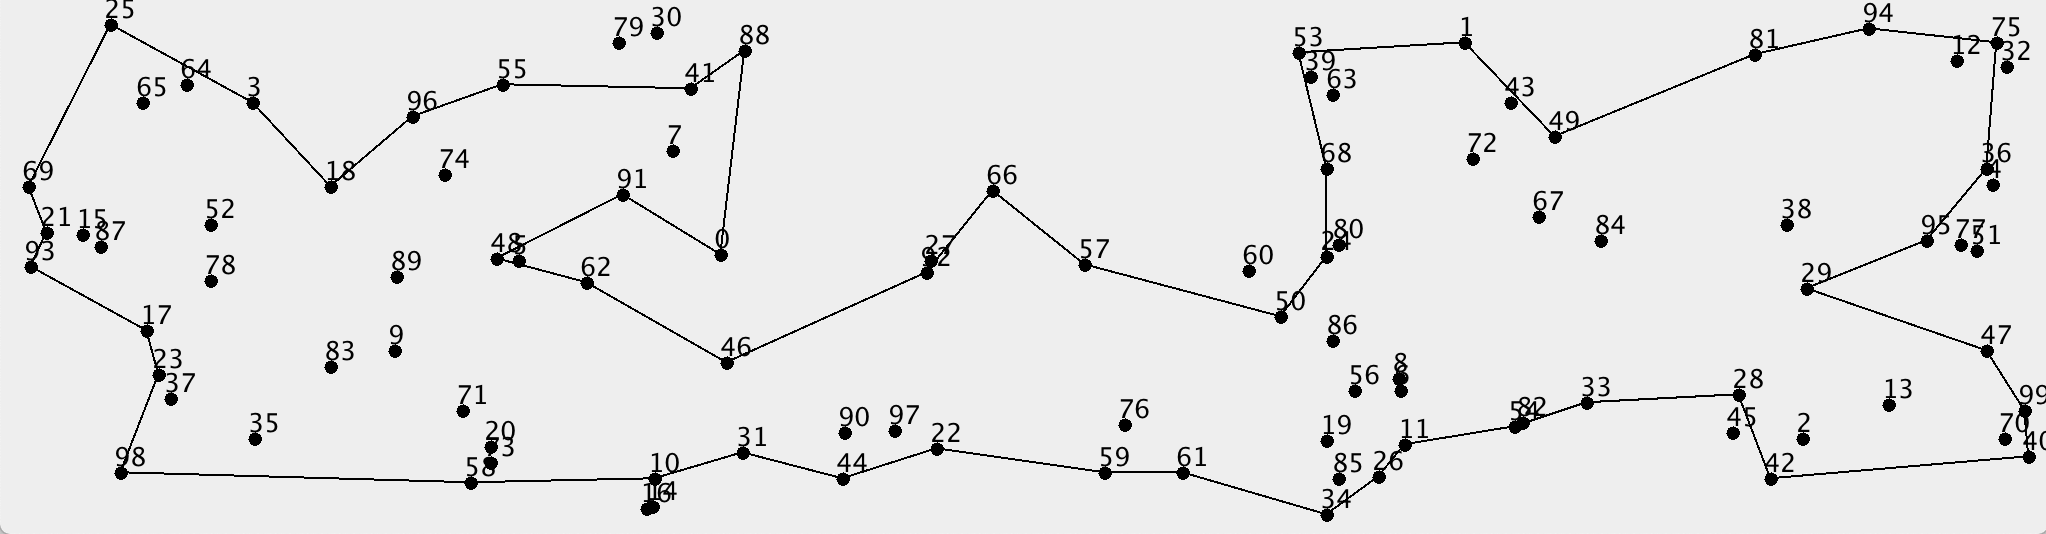
\includegraphics[width=\textwidth]{lab1/kroA_regret}
\caption{Algorytm oparty o żal dla problemu kroA100}
\end{figure}

\subsubsection{Algorytm zachłanny dla problemu kroB100}

\begin{figure}[H]
\centering
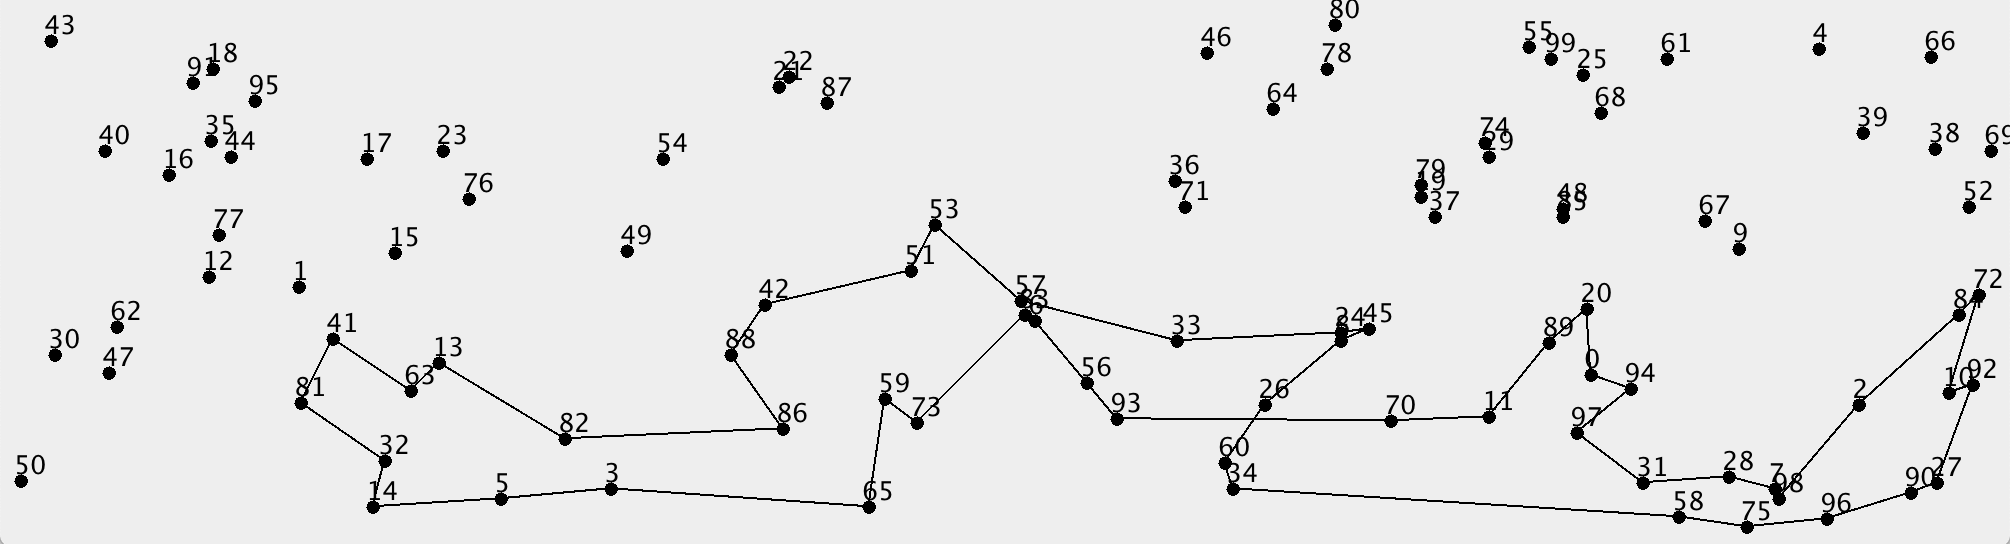
\includegraphics[width=\textwidth]{lab1/kroB_greedy}
\caption{Algorytm zachłanny dla problemu kroB100}
\end{figure}

\subsubsection{Algorytm oparty o żal dla problemu kroB100}

\begin{figure}[H]
\centering
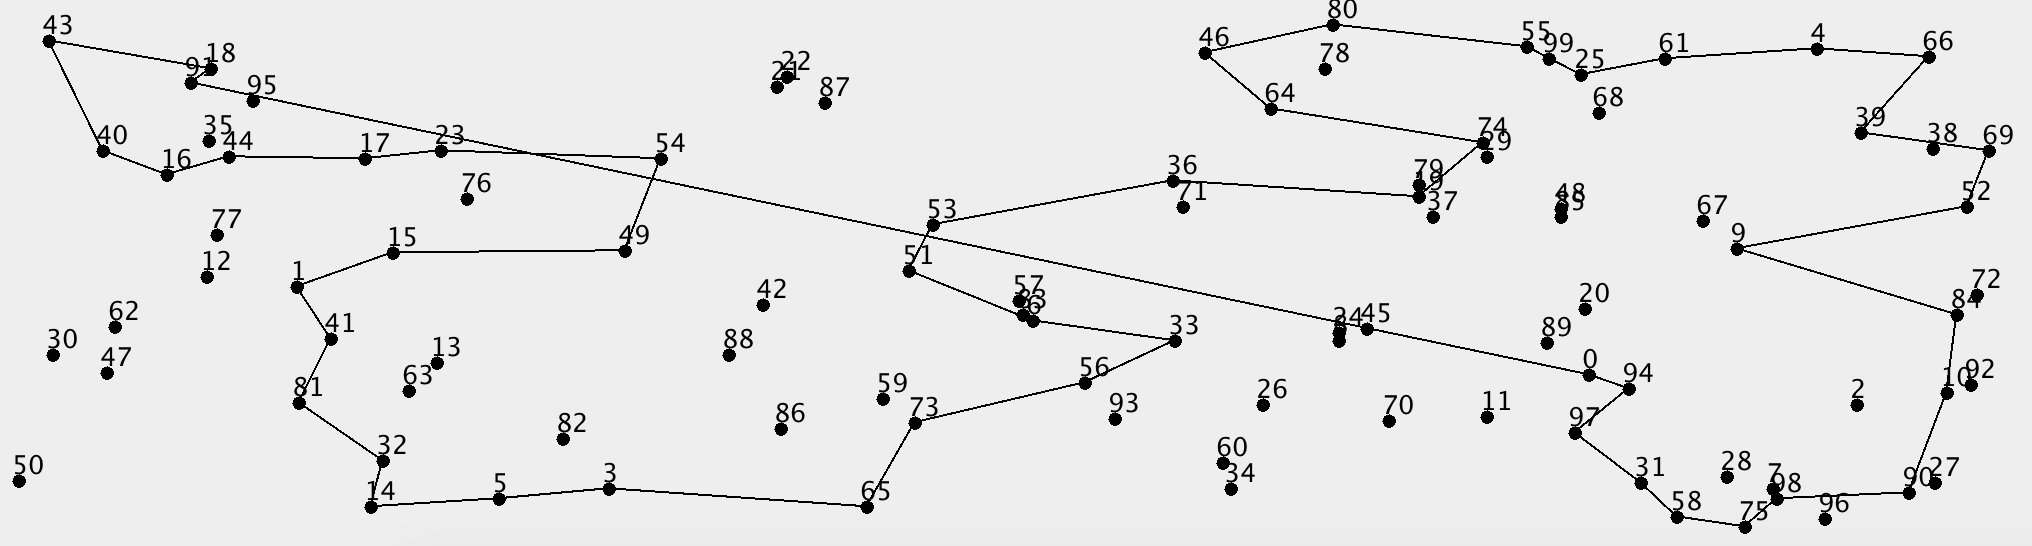
\includegraphics[width=\textwidth]{lab1/kroB_regret}
\caption{Algorytm oparty o żal dla problemu kroB100}
\end{figure}

\subsection{Wnioski}
\paragraph{}
Z wymienionych wyżej pomiarów można wywnioskować, że dla podanych warunków problemu (odwiedzanie połowy punktów), algorytm zachłanny radzi sobie lepiej od algorytmu opartego o żal (cykl, który generuje ma mniejszą długość). Przeprowadzono również testy dla przypadku, gdy oba te algorytmy uruchomione zostaną dla wszystkich punktów. Wtedy wyniki są odmienne, algorytm z żalem okazuje się lepszy od algorytmu zachłannego. Jest to spowodowane tym, że dla warunków zadania z odwiedzeniem połowy punktów algorytm z żalem czasami dodaje punkty, które mają duży żal, a w ogóle nie powinny zostać dodane do cyklu z powodu dużego kosztu ich dodania. Gdy odwiedzone mają być wszystkie punkty, koszt dodania punktu nie ma takiego znaczenia, ponieważ prędzej lub później i tak każdy punkt będzie musiał zostać dodany.

\section{Kod programu}
\paragraph{}
Repozytorium z kodem programu dostępne jest pod adresem: \url{https://github.com/adrianstepienfsw/AEM1}

\end{document}